% multi: https://texblog.org/2012/12/21/multi-column-and-multi-row-cells-in-latex-tables/

% Mit pdflatex mindestens 2mal uebersetzen und Ergebnis mit einem pdf-Viewer betrachten
%\documentclass{beamer}
% https://en.wikibooks.org/wiki/LaTeX/Colors
\documentclass[usenames,dvipsnames,handout]{beamer}
%\usepackage[latin1]{inputenc}
%\usepackage[ngerman]{babel}
\usepackage[utf8]{inputenc}
\usepackage[ngerman]{babel} 
\usepackage{color}
\usepackage{multirow,array}
\usepackage{amsfonts}
\usepackage{amssymb}
%\usepackage{multirow}
\usepackage{hyperref}
\usepackage{tikz}
\usetikzlibrary{shapes.geometric, arrows}
\usetikzlibrary{fit,arrows,calc,positioning}
% http://tex.stackexchange.com/questions/33231/how-to-change-the-color-of-a-block-within-a-custom-beamer-sty-theme-file
\usepackage{color}
\definecolor{mygreen}{cmyk}{0.82,0.11,1,0.25}
\usetheme[secheader]{Boadilla}
\newenvironment{variableblock}[3]{%
  \setbeamercolor{block body}{#2}
  \setbeamercolor{block title}{#3}
  \begin{block}{#1}}{\end{block}}


\begin{document}
\author[Dr. Mariana Nold]{Dr. Mariana Nold}
% \begin{center}
\institute[Institut für Soziologie]{ Institut für Soziologie,\\ Fakultät für Sozial- und Verhaltenswissenschaften,\\ Lehrstuhl für
 empirische Sozialforschung und Sozialstrukturanalyse}
% \end{center}
 \date{}
\title [Punktschätzer und Konfidenzintervalle ]{Punktschätzer und Konfidenzintervalle }
\date{27. November 2017}
\begin{frame}
\maketitle

  \begin{figure}[ht]
 	\centering
 	      
\includegraphics[width=0.15\textwidth]{index.jpeg}
 	\end{figure}
\end{frame} 

\begin{frame}
  \frametitle{Übersicht}
  \tableofcontents
\end{frame}






%http://www.statmethods.net/stats/power.html
\section{Ziel der heutigen Veranstaltung}
\begin{frame}{Ziel der heutigen Veranstaltung \dots}
ist es die folgenden Fragen beantworten zu können:
\begin{block}{Zielfragen für heute}
\begin{enumerate}
\item{Welche Probleme treten auf, wenn man den Fehler 2. Art nicht berücksichtigt?}
\item{Wie ist die Power eines Tests definiert?}
\item{Wie ist die Schätzstatistik definiert?}
\item{Welche Punktschätzung verwendet man für Anteilswerte?}
\item{Was ist der Standardfehler?}
\item{Warum braucht man die Intervallschätzung?}
\item{Was versteht man unter eine Konfidenzintervall und wie interpretiert man es?}
\item{Wie sieht das Konfidenzintervall für Anteilswerte aus?}
\end{enumerate}
\end{block}
\end{frame}
\section{Stichprobenumfang und Power}
\subsection{Kritik am klassischen statistischen Testen }
%
\begin{frame}{Kritik am klassischen statistischen Testen }
(vgl. LMLG S. 136 ff und 166 ff)
\begin{itemize}
\item{Statistisches Testen spielt in der Praxis der empirischen Sozialforschung einer herausragende Rolle.}\pause
\item{Tatsächlich ist sowohl das Konzept der statistischen Signifikanz als auch die Logik des statistischen
Testens überhaupt seit Jahrzehnten der Kritik ausgesetzt.}\pause
\item{Immer wieder haben renommierte Wissenschaftler gefordert, man solle statistische Signifikanztests
abschaffen. }\pause
\item{Ich möchte heute einen Kritikpunkt vorstellen und eine Möglichkeit die mit weniger Nachteilen
verbunden ist.}
\end{itemize}
\end{frame}
\begin{frame}{Die Füllmenge der Flaschen}
\begin{itemize}
\item{In der Aufgabe 6 des letzten Aufgabenblattes ging es um die Frage, ob eine Maschine die 
Mineralwasserflaschen befüllt  neu eingestellt werden muss.}\pause
\item{Die Maschine soll exakt
$500$ ml pro Flasche abfüllen. Nehmen wir an, der wahre Mittelwert der Füllmenge
ist $\mu$ und die wahre Standardabweichung $\sigma.$ Beide Parameter sind
unbekannt. Der Stichprobenumfang ist $n.$}\pause
\item{Wir wollen uns heute zunächst mit dem Fehler 2. Art beschäftigen.  Also mit dem Fehler eine unwahre 
Nullhypothese nicht zu erkennen und beizubehalten.}
\item{Es kann auch passieren, dass ein relevanter Unterschied nicht signifikant ist. Dass ist dann ein Fehler 2. Art.}
\end{itemize}
\end{frame}

\begin{frame}{Wie falsch darf die Maschine arbeiten?}
\begin{itemize}
\item{Die Toleranz wird auf $20$ ml in beide Richtungen festgelegt. Das bedeutet:
Eine Akzeptable Füllmenge liegt im Intervall $(480,520).$}\pause
\item{Die Instandsetzung der Maschine zur Neuadjustierung der Füllmenge kostet $200$ Euro.
Daher möchte die Mitarbeiterin diese nur vornehmen, wenn sie auch nötig ist.}\pause
\item{Da eine Abweichung der Füllmenge sowohl nach oben, als auch nach unten
zu Problemen führt, arbeiten mir mit der ungerichteten Null-Hypothese $H_{0}: \mu=\mu_{0}=500$}\pause
\item{Wenn also die wahre erwartete Füllmenge $490$ ml beträgt und der Test diese
Abweichung erkennt und $H_{0}$ ablehnt, dann entsteht ein Schaden von $200$ Euro.}
\end{itemize}
\end{frame}

\begin{frame}{Der Test kennt keinen Toleranzbereich}
\begin{itemize}
\item{Bitte beachten Sie: Die Nullhypothese ist schon bei der geringsten Abweichung nicht mehr
wahr. Selbst, wenn die Maschine eine erwartete Füllmenge von $503$ ml hat, ist die Nullhypothese
tatsächlich falsch.}
\item{Ein Kritikpunkt an der Praxis des statistischen Testens ist daher, dass man unterscheiden
sollte zwischen \textbf{relevanten} und \textbf{signifikanten} Unterschieden.}
\item{Es kann passieren, dass ein nicht relevanter Unterschied als signifikant nachgewiesen wird.
Das ist kein Fehler, weder ein Fehler 1. Art, noch ein Fehler 2. Art.}
\end{itemize}
\end{frame}
\subsection{Kein guter Test ohne Berücksichtigung der Power}
\begin{frame}{Power oder Stärke eines statistischen Tests}
Um zu verstehen, wie man einen statistischen Test richtig anwenden sollte, brauchen wir den 
Begriff der Power.\pause
\begin{variableblock}{Definition: Power oder Stärke eines statistischen Tests}{bg=Orchid!30,fg=black}{bg=Plum!30,fg=black}
Die Stärke eines statistischen Tests ist dessen Fähigkeit, einen in der Grundgesamtheit vorhandenen
Unterschied (oder eine andere Größe, die wir testen wollen) auch tatsächlich zu ermitteln.\\

Es gilt also: Power= 1-$\beta$ (Wahrscheinlichkeit des Fehlers 2. Art), eine hohe Power bedeutet also ein kleines
Risiko, einen Fehler 2. Art zu begehen. Eine hoher Power bedeutet aber auch ein hohes Risiko nicht relevante
Unterschiede als signifikant nachzuweisen.
\end{variableblock}
\end{frame}

\begin{frame}{Die Power und der Stichprobenumfang}
\begin{itemize}
\item{Desto höher der Stichprobenumfang ist, desto mehr empirischen Information liegt vor. Daher steigt die
Power eines Tests mit dem Stichprobenumfang.}\pause
\item{In Aufgabe 6 hatte die Mitarbeiterin 20 Flaschen getestet. Ist das ein gute Anzahl?
Wird durch diese Anzahl ein relevanter Unterschied nachweisbar?}
\item{Um diese Frage zu diskutieren, gehen Sie bitte davon aus, dass die Standardabweichung der Maschine $20$ ml beträgt.
Dieser Wert ist der Mitarbeiterin allerdings nicht bekannt.}
\end{itemize}
\end{frame}

\begin{frame}{Wie hoch ist die Power des einfachen t-Test?}
\begin{itemize}
\item{Die erwartete  Füllmenge, die wir testen wollen heißt $\mu_{0}$}\pause
\item{Die uns unbekannte wirkliche erwarte Füllmenge heißt $\mu.$}\pause
\item{Die wahre Füllmenge ist normalverteilt mit den Parameter $\mu$ und $\sigma.$}\pause
\item{Die Power dieses Test hängt von der Effektgröße $$\delta:=\frac{\mu-\mu_{0}}{\sigma}$$ ab.}\pause
\item{Für unser Beispiel gilt: $$\delta:=\frac{\mu-500}{20}$$}\pause
\item{Wie viele Flaschen sollte die Mitarbeiterin für Ihren Test verwenden?}\pause
\item{Wie viele Flaschen sollte Sie verwenden, wenn schon eine Abweichung von $10$ ml relevant wäre?}
\end{itemize}
\end{frame}

\begin{frame}{Was ist ein relevanter Unterschied?}
\begin{itemize}
\item{Die erlaubte Toleranz sind $20$ ml, also genau eine Standardabweichung.
Der Idealfall wäre, wenn der Test nur signifikant ist, wenn die Füllmenge
außerhalb des Intervalls $(480,520)$ liegt.}\pause
\item{Wenn man dieses Intervall auf die Effektgröße umrechnet, erhält man 
das Intervall $(-1,1).$}
\item{Die Grafik auf der nächsten Folie zeigt die Power des einfachen t-Test bei ungerichtete Nullhypothese $\mu=\mu_{0}=500$
für unterschiedliche Stichprobenumfänge.}
\end{itemize}
\end{frame}

\begin{frame}{Power für die Nullhypothese $\mu=\mu_{0}=500$}
  \begin{figure}[ht]
 	\centering
 	      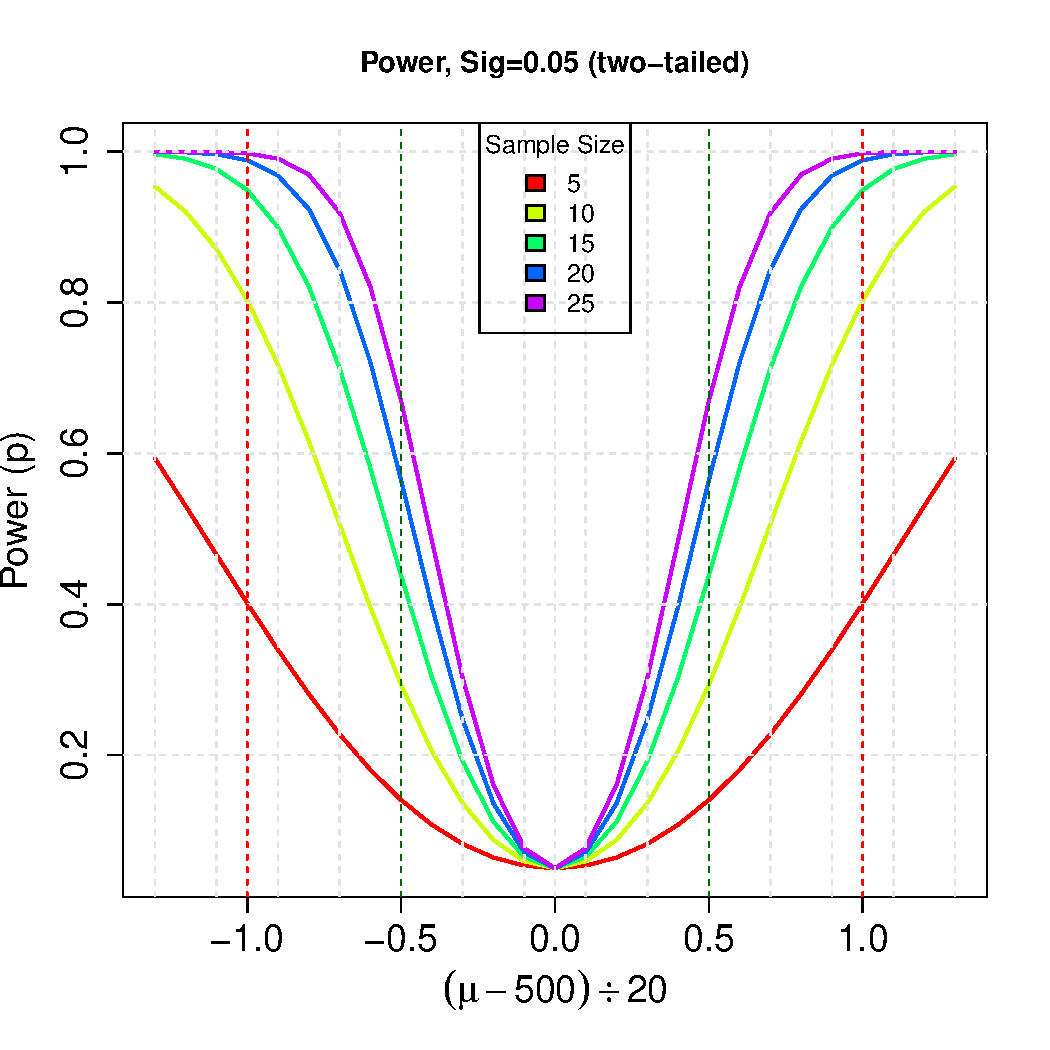
\includegraphics[width=0.65\textwidth]{power3.pdf}%{overlap3.pdf}
 	\end{figure}
\end{frame}

\begin{frame}{Ein zu großer Stichprobenumfang? }
  \begin{figure}[ht]
 	\centering
 	      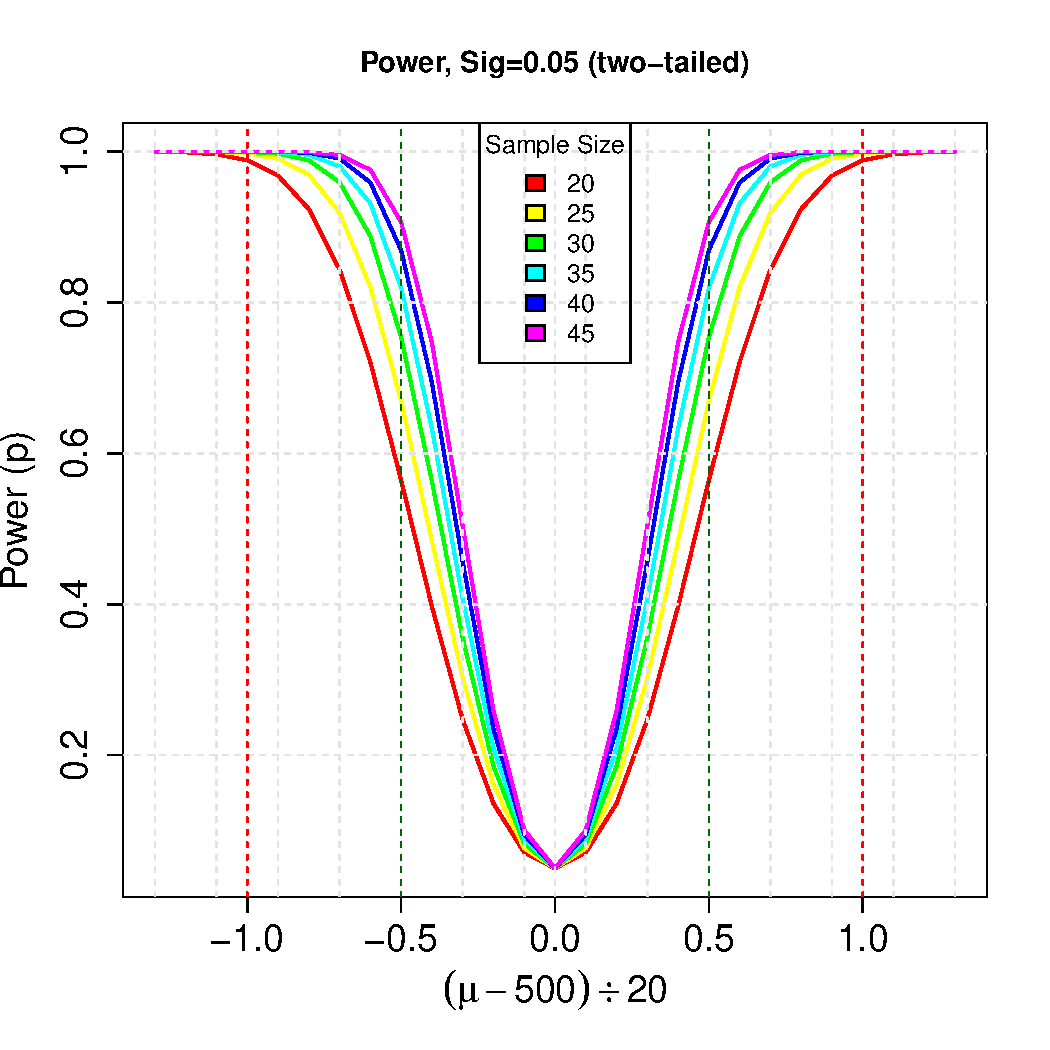
\includegraphics[width=0.65\textwidth]{power4.pdf}%{overlap3.pdf}
 	\end{figure}
\end{frame}

\begin{frame}{Statistische Tests unter Berücksichtigung der Teststärke (vgl. LMLG S. 171)}
Statistisches Testen, das unter Berücksichtigung der Ideen von Neyman und Pearson auf die Teststärke 
achtet, muss
\begin{itemize}
\item[1)]{der Nullhypothese eine eindeutige Alternativhypothese gegenüber stellen.}
\item[2)]{mit Blick auf diese Alternativhypothese (was ist relevant?) den Stichprobenumfang so
anpassen,}
\item[3)]{dass eine zufriedenstellende Teststärke erzielt wird.}
\end{itemize}\pause
Es gibt statistische Software, die die Power  für viele Tests berechnet. Es ist allerdings
die Ausnahme, dass jemand solche Software verwendet.
\end{frame}
%http://sites.nicholas.duke.edu/statsreview/ci/
%https://www.r-bloggers.com/demonstrating-confidence-intervals-with-shiny/
\begin{frame}{Statistisches Testen}
\begin{itemize}
\item{Eine vollständige Diskussion mit den Pro und Kontra-Punkten für und gegen das 
statische Test, können wir hier nicht führen.}
\item{Die bisherigen Folien geben nur einen kleinen Einblick.}
\item{Im Rest der Veranstaltung wollen wir uns mit Punktschätzern und Konfidenzintervallen
beschäftigen.}
\item{Die Auswertung der Daten mit Hilfe von Punktschätzern und Konfidenzintervallen
ist klar im Vorteil gegenüber statistischen Tests.}
\end{itemize}
\end{frame}
% Tolles Bild
%http://www.statistik-und-beratung.de/2013/07/statistischer-vergleich-von-zwei-gruppen/
\begin{frame}{Ausblick Übung: Lesen Mädchen besser als Jungs?}
\begin{itemize}
\item{In Aufgabe $5$ des Aufgabenblattes $2,$ konnten Sie mit dem doppelten t-Test nachweisen,
dass Mädchen besser lesen als Jungen.}\pause
\item{Bisher haben wir bei diesem Test die Teststärke nicht berücksichtigt, dass soll in der nächsten
Übung erfolgen.}\pause
\item{Ist der signifikante Unterschied auch relevant? }\pause
\item{Das Effektmaß $\delta$ des doppelten t-Tests ist: $$\delta:=\frac{\mu_{X}-\mu_{Y}}{\sigma},$$
wobei $\mu_{X}$ der Erwartungswert der Lesepunkte der Mädchen ist und 
$\mu_{Y}$ der Erwartungswert der Lesepunkte der Jungen. Die Standradabweichung innerhalb der 
Gruppen wird als homogen angenommen und mit $\sigma$ bezeichnet. }
\end{itemize}
\end{frame}

\begin{frame}{Übung: Lesen Mädchen besser als Jungs? }
  \begin{figure}[ht]
 	\centering
 	      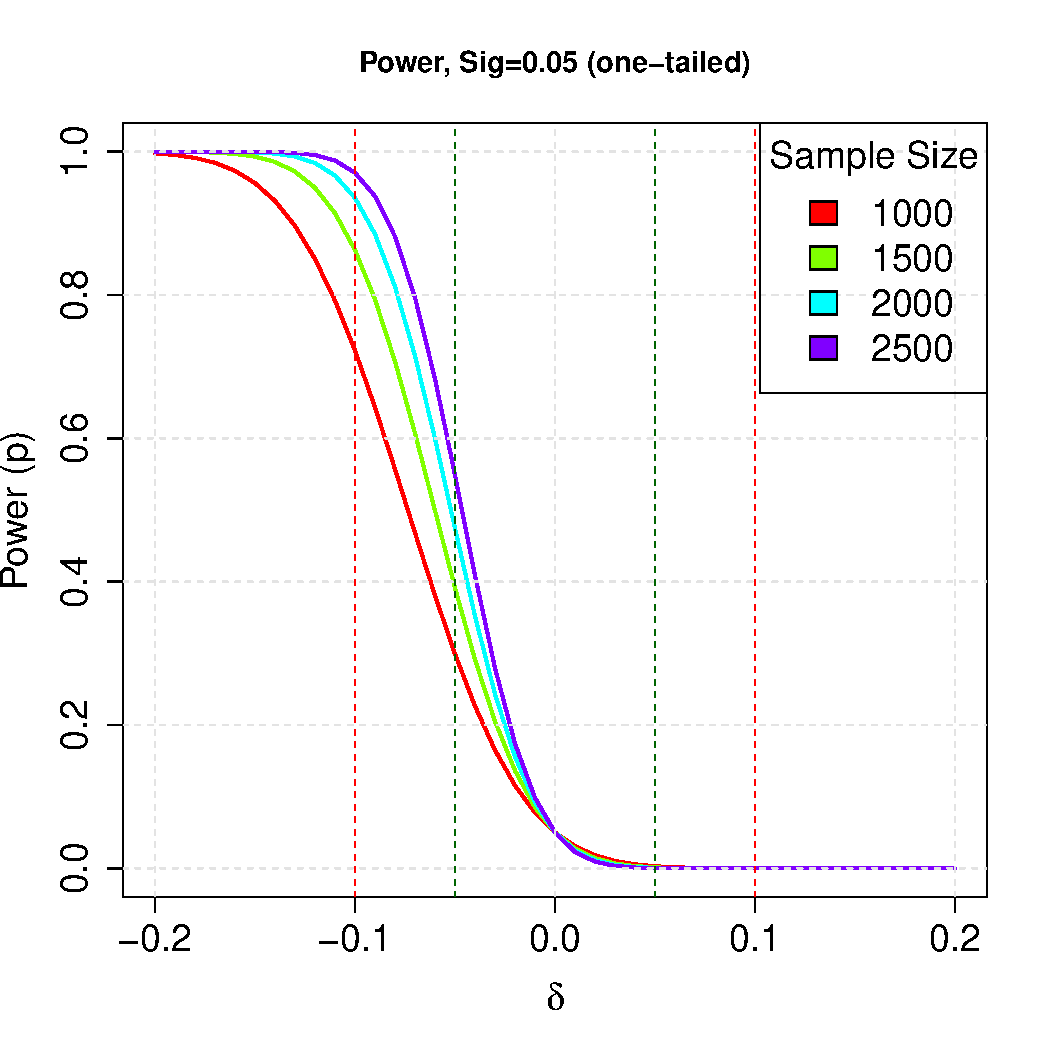
\includegraphics[width=0.65\textwidth]{powerPisa.pdf}%{overlap3.pdf}
 	\end{figure}
\end{frame}

\section{Punktschätzer und Intervallschätzer für den Anteilswert}
\subsection{Beispiel: Die diffusen Ängste der Deutschen}
\begin{frame}{Die diffusen Ängste der Deutschen (17.2.16)}
%http://www.faz.net/aktuell/politik/inland/allensbach-umfrage-zeigt-angst-um-innere-sicherheit-steigt-14073805/infografik-sorgen-um-die-14074061.html
  \begin{figure}[ht]
 	\centering
 	      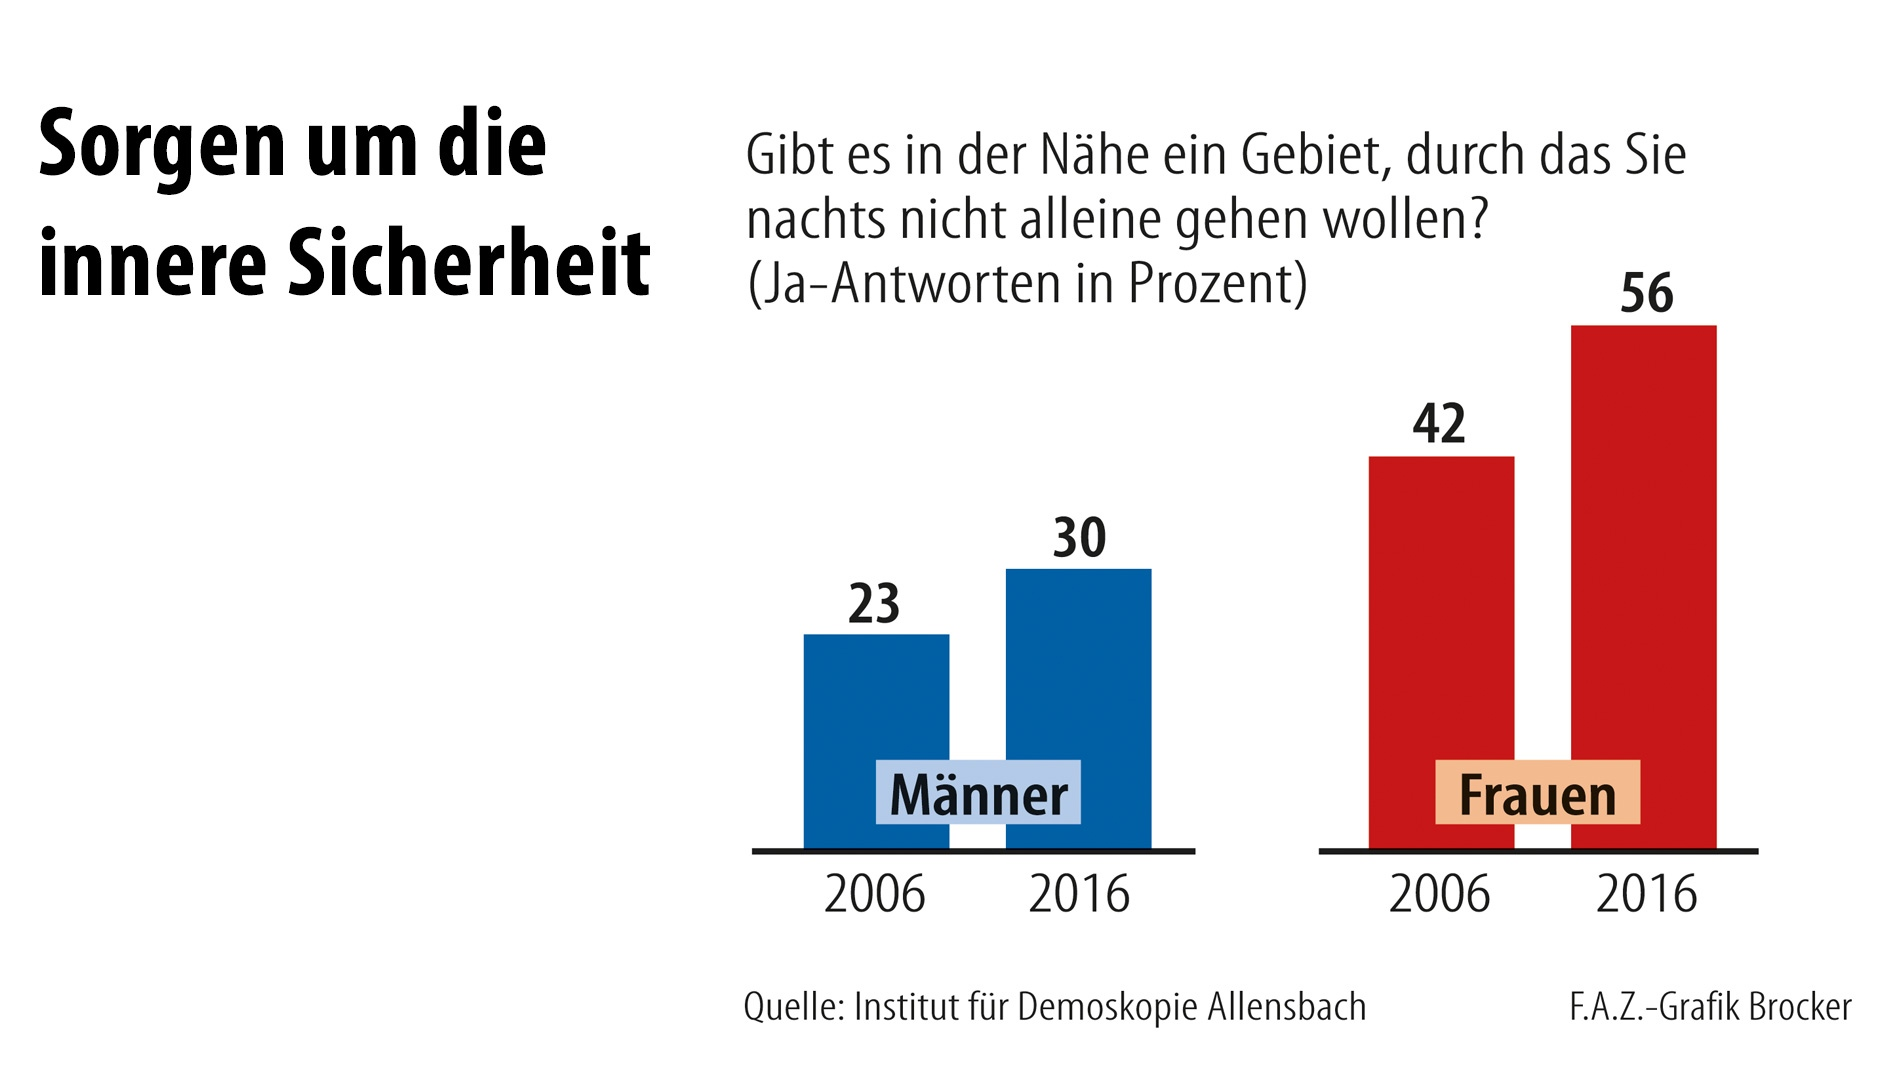
\includegraphics[width=0.85\textwidth]{sorgen.jpg}%{overlap3.pdf}
 	\end{figure}
\end{frame}

%\begin{frame}{Untersuchungsdaten: Allensbach-Umfrage}
%\begin{itemize}
%\item{ 
%Befragter Personenkreis:
%Deutsche Wohnbevölkerung ab 16 Jahre in 
%der Bundesrepublik Deutschland}
%\item{Anzahl der Befragten:
%1521
%Befragungszeitraum:
%01. Februar bis 11. Februar 2016}
%\item{Methode:
%Repräsentative Quotenauswahl
%Art der Interviews:
%Mündlich-persönliche Interviews}
%\end{itemize}
%\end{frame}
\begin{frame}{Definition der Zufallsvariablen $X_{i}$}
\begin{description}
\item{Die Grundgesamtheit für die wir uns im Folgenden interessieren ist, die der deutschen Männer im Jahr $2016.$}
\item{Wie hoch ist der Anteil der besorgten Männer in der Grundgesamtheit? }
\item{Wir nennen $X_{i}$ die Antwort  des $i$ ten Mannes in der Befragung.}
\end{description}
Es ist
     \[
     X_{i}:=\left\{\begin{array}{ll} 0, \: \text{``nein,''} \\
        1, \:  \text{``ja''}\end{array}\right. 
  \]
  je nachdem ob der $i$-te Mann in der Stichprobe ablehnt oder zustimmt.
\end{frame}

\begin{frame}{Die Stichprobenvariablen} %FT S. 365
\begin{itemize}
\item{Ausgangspunkt der Punktschätzung sind $n$ Stichprobenziehungen oder Zufallsexperimente, die durch Zufallsvariablen 
$X_{1}, \dots X_{n}$ repräsentiert werden.}\pause
\item{$X_{1}, \dots X_{n}$ werden auch als Stichprobenvariablen bezeichnet.}\pause
\item{Häufig fordert man von Stichprobenfunktionen, dass sie unabhängige Wiederholungen von $X$ sind. Durch diese
knappe Formulierung wird ausgedrückt, dass
\begin{itemize}
\item{die den Zufallsvariablen $X_{1}, \dots X_{n}$ zugrundeliegenden Experimenten unabhängig sind,}
\item{jedes mal dasselbe Experiment (enthalten in ``Wiederholung'') durchgeführt wird.}
\end{itemize}}\pause
\item{Man kürzt diese Annahme mit iid-Annahme ab.}
\end{itemize}
\end{frame}

\begin{frame}{Der (Punkt)Schätzer}
Der etablierte Schätzer für den Anteil $p$ in der Grundgesamtheit ist $$\hat{p}=\bar{X}=\sum_{i=1}^{n} x_{i}.$$\pause
 Allgemein gilt:
\begin{variableblock}{Definition: Punktschätzer, Schätzfunktion, Schätzstatistik}{bg=Orchid!30,fg=black}{bg=Plum!30,fg=black}
Ein Punktschätzer für den Grundgesamtheitsparameter $\theta$ ist eine Funktion
$$T=\hat{\theta}=g(X_{1}, \dots X_{n}) $$  der Variablen $X_{1}, \dots X_{n}.$ Der aus den Realisationen 
$x_{1}, \dots x_{n}$ resultierende numerische Wert
$$t=\hat{\theta}=g(x_{1}, \dots x_{n}) $$   ist der zugehörige Schätzwert.
\end{variableblock}
\end{frame}

\begin{frame}{Erwartungstreue  (vgl. FS. 49)}
Die Punktschätzer, die wir in diesem Semester behandeln, sind erwartungstreu.
\begin{variableblock}{Definition: Erwartungstreue}{bg=Orchid!30,fg=black}{bg=Plum!30,fg=black}
Eine Schätzstatistik $\hat{\theta}=g(X_{1}, \dots X_{n})$ heißt erwartungstreu für $\theta,$ wenn gilt
%$\mathbb{Z}$
$$ \mathbb{E}_{\theta} (\hat{\theta}) = \theta.$$
\end{variableblock}\pause
Der Erwartungswert ist ein  Lagemaß
für die Verteilung von Zufallsvariablen.
Der Erwartungswert einer Zufallsvariable wird gebildet indem man die Werte die die Zufallsvariable annehmen kann mit der entsprechenden
Wahrscheinlichkeit gewichtet.\\
Daher ist die Forderung der Erwartungstreue eine sehr naheliegende und sinnvolle  Forderung an einen Schätzer.
%\begin{itemize}
%\item[1)]{Bei stetigen Zufallsvariablen entspricht das mathematisch einer Integration. }
%\item[2)]{Bei diskreten Zufallsvariablen ist die Berechnung sehr ähnlich zur Berechnung des Mittelwertes. Man gewichtet die Ausprägung mit der Wahrscheinlichkeit.}
%\end{itemize}
\end{frame}

\begin{frame}{Interpretation Erwartungstreue}
\begin{itemize}
\item{Wichtig ist das Verständnis, dass  der Erwartungswert eine wichtiges Lagemaß für eine Zufallsvariable ist.}\pause
\item{Wenn die Zufallsvariable eine Schätzstatistik ist, dann gibt ihr Erwartungswert die zentrale Tendenz
dieser Schätzstatistik  wieder.}\pause
\item{In einfachen Worten bedeutet das: Man erwartet, dass die Realisation der Schätzstatistik dem wahren Parameter
entspricht, wenn Erwartungstreue vorliegt.}
\end{itemize}
\end{frame}

\begin{frame}{Punktschätzer und Intervallschätzer für den Anteilswert}
\begin{itemize}
\item{Wir gehen im Folgenden von einer iid Stichprobe aus. $X_{i}$ iid wie $X \sim Be(p).$}\pause
\item{Bei der Punktschätzung geht es darum, einen Parameter in der Grundgesamtheit
zu schätzen. }\pause
\item{Der entspreche Anteil in der Stichprobe ist $30\%.$}\pause
\item{Der Schätzer $\hat{p}$
für den Anteil $p$ der besorgten Männer in der Grundgesamtheit ist daher $0.3.$}\pause
\item{Wir schätzen also diesen Anteil in der  Grundgesamtheit auf $30\%.$ Aber wie präzise ist die Schätzung?}\pause
\item{Kann es sein, dass es in Wirklichkeit nur $10\%$ sind oder gar $50\%$?}
\end{itemize}
\end{frame}
\begin{frame}{Warum brauchen wir die Intervallschätzung}%FT S. 385
\begin{itemize}
\item{Die Punktschätzung liefert einen Schätzer $\hat{\theta}$ im konkreten Beispiel $\hat{p}.$}
\item{Dieser ist im Regelfall nicht mit dem wahren Parameter $\theta$ bzw. $p$ identisch.}\pause
\item{In jeder sinnvollen Anwendung ist es daher notwendig, neben dem Schätzwert selbst, die Präzision
des Schätzverfahren mitanzugeben.}\pause
\item{Ein Maß für die Präzision ist der Standardfehler, allerdings nur bei erwartungstreuen Schätzern
mit symmetrischer Verteilung. }\pause
\item{Ein anderer Weg die Genauigkeit des Schätzverfahren direkt miteinzubeziehen, ist die 
Intervallschätzung.}\pause
\item{Das Ergebnis der der Intervallschätzung ist nicht ein Wert sondern ein Intervall.}\pause
%\item{Wie diese Intervalle berechnet werden entnimmt man der Formelsammlung bzw.
%man lässt \texttt{STATA} oder eine andere Statstik-Software rechnen.}
\end{itemize}
\end{frame}
% eigentlich kennen sie beides schon
% annahme es wären 100 befragte

% siehe confi3.r
\begin{frame}{Ein Konfidenzintervall für den Anteilswert}
Das approximative $(1-\alpha)$-Konfidenzintervall für den Anteil $p$ in einer Grundgesamtheit ist
\begin{equation}
\label{eq:1}
\bigg[\hat{p} - z_{1-\frac{\alpha}{2}}\Bigg(\sqrt{\frac{\hat{p}(1-\hat{p})}{n}}\Bigg),\hat{p} + z_{1-\frac{\alpha}{2}}\Bigg(\sqrt{\frac{\hat{p}(1-\hat{p}}{n}}\Bigg) \Bigg],
\end{equation}
 wobei $z_{1-\frac{\alpha}{2}}$ das $(1-\alpha)$-Quantil der Standardnormalverteilung ist.\pause
\begin{itemize}
\item{Man kann mit \texttt{STATA} oder andere Statistik-Software eine Intervallschätzung
für eine vorher festgelegtes Konfidenzniveau $\alpha$ berechnen.}
\item{Sie können dieses Konfidenzintervall interpretieren, als ein Intervall,
dass alle Nullhypothesen enthält, die der approximative Binomialtest mit Irrtumswahrscheinlichkeit $\alpha$ beibehält.}\pause
%\item{Wenn man eine Stichprobe von  $100$ Männern hat, von denen $30$ die Frage bejahen, ergibt sich 
%$[0.22,0.40]$ }\pause
%\item{Wenn man eine Stichprobe von  $1000$ Männern hat, von denen $300$ die Frage bejahen, ergibt sich 
%$[0.27,0.33]$ }

\end{itemize}
\end{frame}
% Chi-Test: Aber wie groß sind die Anteilswerte? -> Übung
% Hatten wir schon gesehen in PISA und eine Interpretation können wir schon sofort angeben

% http://www.faz.net/aktuell/politik/inland/allensbach-umfrage-zeigt-angst-um-innere-sicherheit-steigt-14073805/infografik-sorgen-um-die-14074061.html
\begin{frame}{Eine zweite Herleitung bzw. Interpretation der Intervallschätzung?}
\begin{itemize}
\item{Im folgenden gehen wir davon aus, dass der wahre (und unbekannte) Anteil der männlichen Personen ab
16 Jahren, die der Frage zustimmen, in der Grundgesamtheit bei $25\%$ liegt.}\pause
%\item{Stellen Sie sich vor wir erheben $100$ Stichproben mit je $100$ Personen aus der Grundgesamtheit.}\pause
\item{Sie können sich vorstellen, dass $k$ Personen losgehen und jede Person eine einfach Zufallsstichprobe mit je
$100$ Personen zieht.}\pause
\item{Wir gehen dabei davon aus, dass die Grundgesamtheit so groß ist, dass keine Person doppelt vorkommt.}\pause
\item{Die Folgenden Grafiken zeigen für $k \in (100,200,250)$
\begin{itemize}
\item[1)]{das Histogramm der  beobachteten Anteilswerte $\hat{p}=\bar{x}$ und}
\item[2)]{die entsprechenden Konfidenzintervalle wie in \eqref{eq:1} (vgl. FS S. 52)}
\end{itemize}
}
\end{itemize}
\end{frame}



\begin{frame}{Beobachtete Anteilswerte $\hat{p}$: $100$ Befragungen}
%http://www.faz.net/aktuell/politik/inland/allensbach-umfrage-zeigt-angst-um-innere-sicherheit-steigt-14073805/infografik-sorgen-um-die-14074061.html
  \begin{figure}[ht]
 	\centering
 	      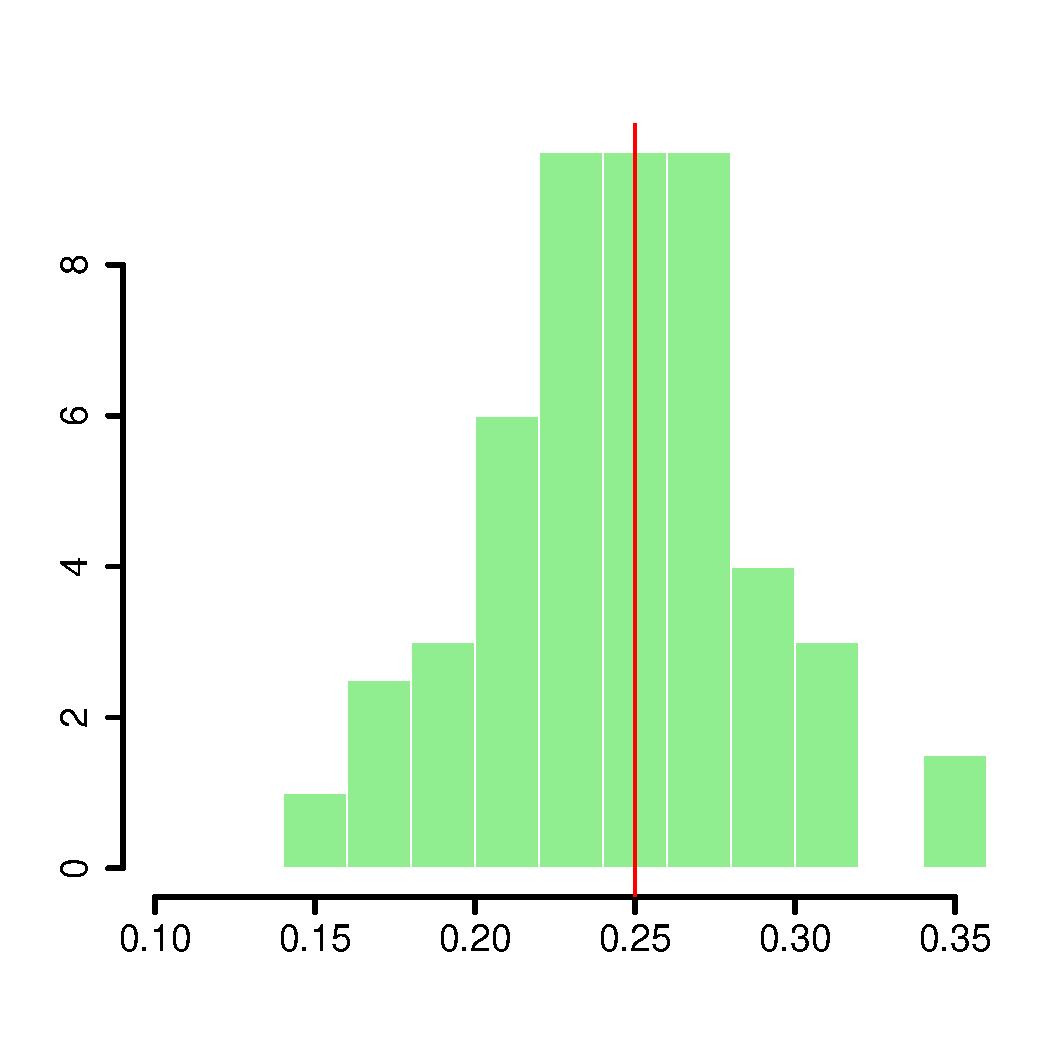
\includegraphics[width=0.65\textwidth]{prob_est.pdf}%{overlap3.pdf}
 	\end{figure}
\end{frame}

\begin{frame}{Konfidenzintervalle zu den Anteilswerten: $100$ Befragungen}
%http://www.faz.net/aktuell/politik/inland/allensbach-umfrage-zeigt-angst-um-innere-sicherheit-steigt-14073805/infografik-sorgen-um-die-14074061.html
  \begin{figure}[ht]
 	\centering
 	      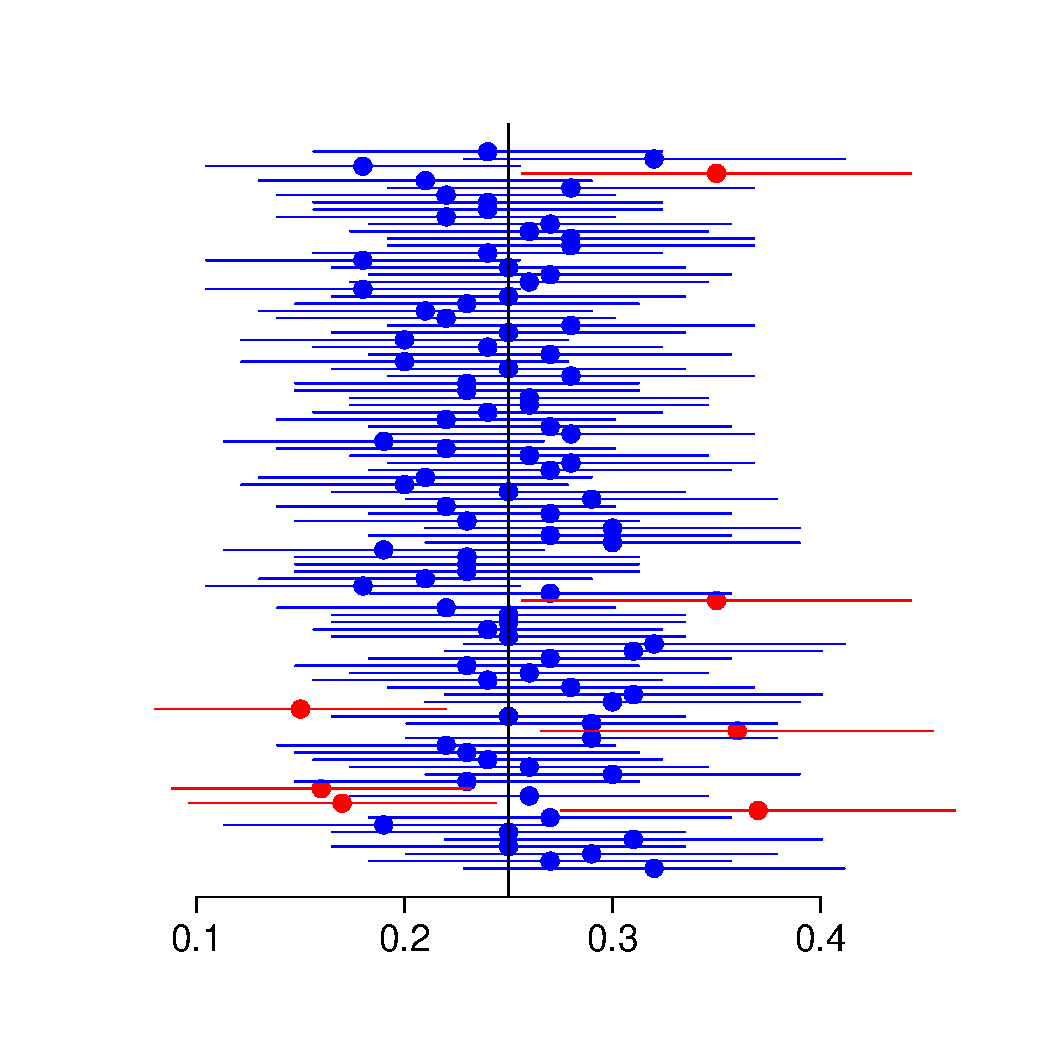
\includegraphics[width=0.65\textwidth]{confi.pdf}%{overlap3.pdf}
 	\end{figure}
\end{frame}

\begin{frame}{Betrachtung der Ergebnisse}
\begin{itemize}
\item{Von den $100$ Personen, die losgegangen sind, um jeweils eine Stichprobe von  $100$ Personen
zu ziehen, haben sieben eine Stichprobe gezogen, deren Konfidenzintervall den wahren Wert nicht
enthält.
}\pause
\item{Die anderen $93$ haben eine Stichprobe gezogen, deren Konfidenzintervall, den wahren Wert enthält.}\pause
\item{Wir wiederholen das Experiment. Diesmal gehen 200 Personen los um jeweils 100 Personen zu befragen.}\pause
\item{Was erwarten Sie? Wie viele Konfidenzintervalle werden den wahren Anteilswert nicht enthalten?}
\end{itemize}
\end{frame}

\begin{frame}{Beobachtete Anteilswerte $\hat{p}$: 200 Befragungen}
%http://www.faz.net/aktuell/politik/inland/allensbach-umfrage-zeigt-angst-um-innere-sicherheit-steigt-14073805/infografik-sorgen-um-die-14074061.html
  \begin{figure}[ht]
 	\centering
 	      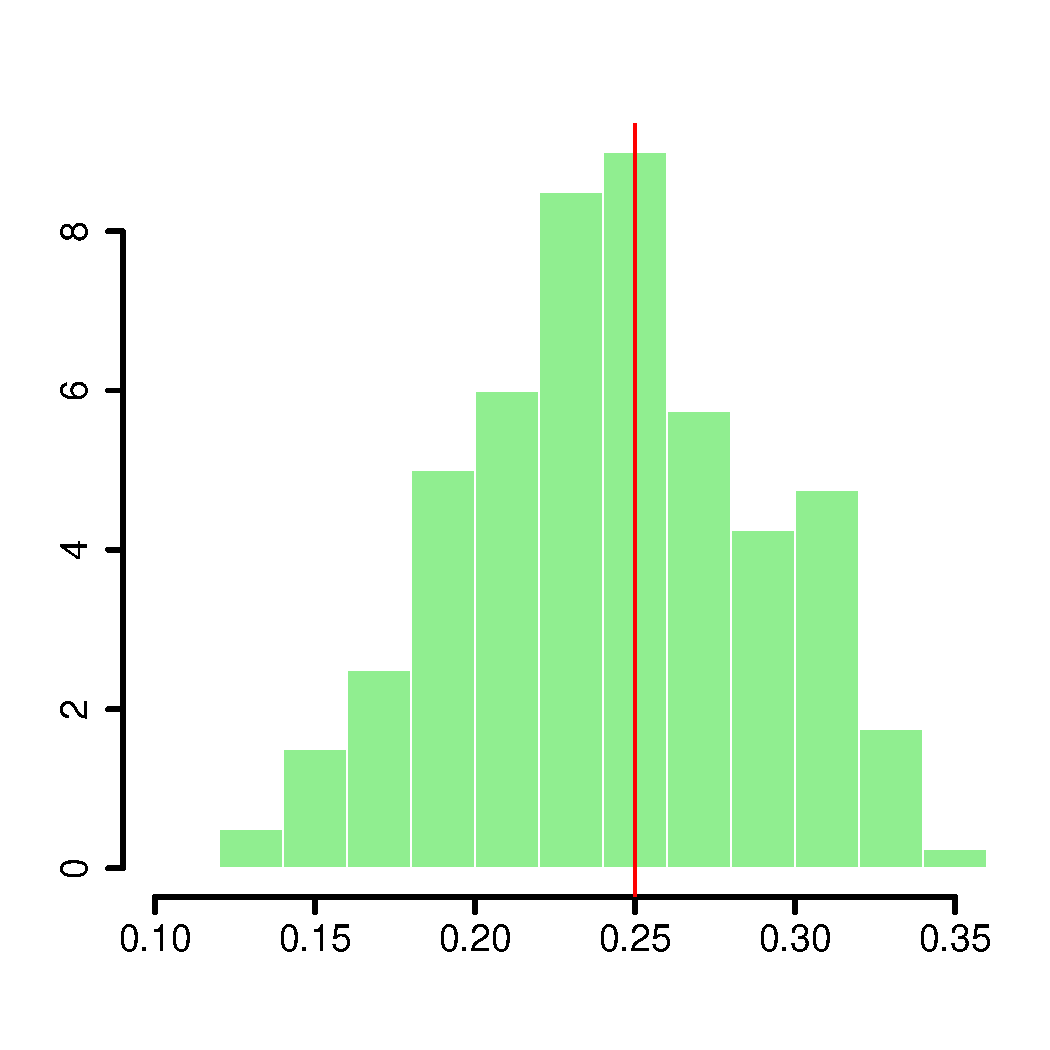
\includegraphics[width=0.65\textwidth]{prob_est200.pdf}%{overlap3.pdf}
 	\end{figure}
\end{frame}

\begin{frame}{Konfidenzintervalle zu den Anteilswerten: 200 Befragungen}
%http://www.faz.net/aktuell/politik/inland/allensbach-umfrage-zeigt-angst-um-innere-sicherheit-steigt-14073805/infografik-sorgen-um-die-14074061.html
  \begin{figure}[ht]
 	\centering
 	      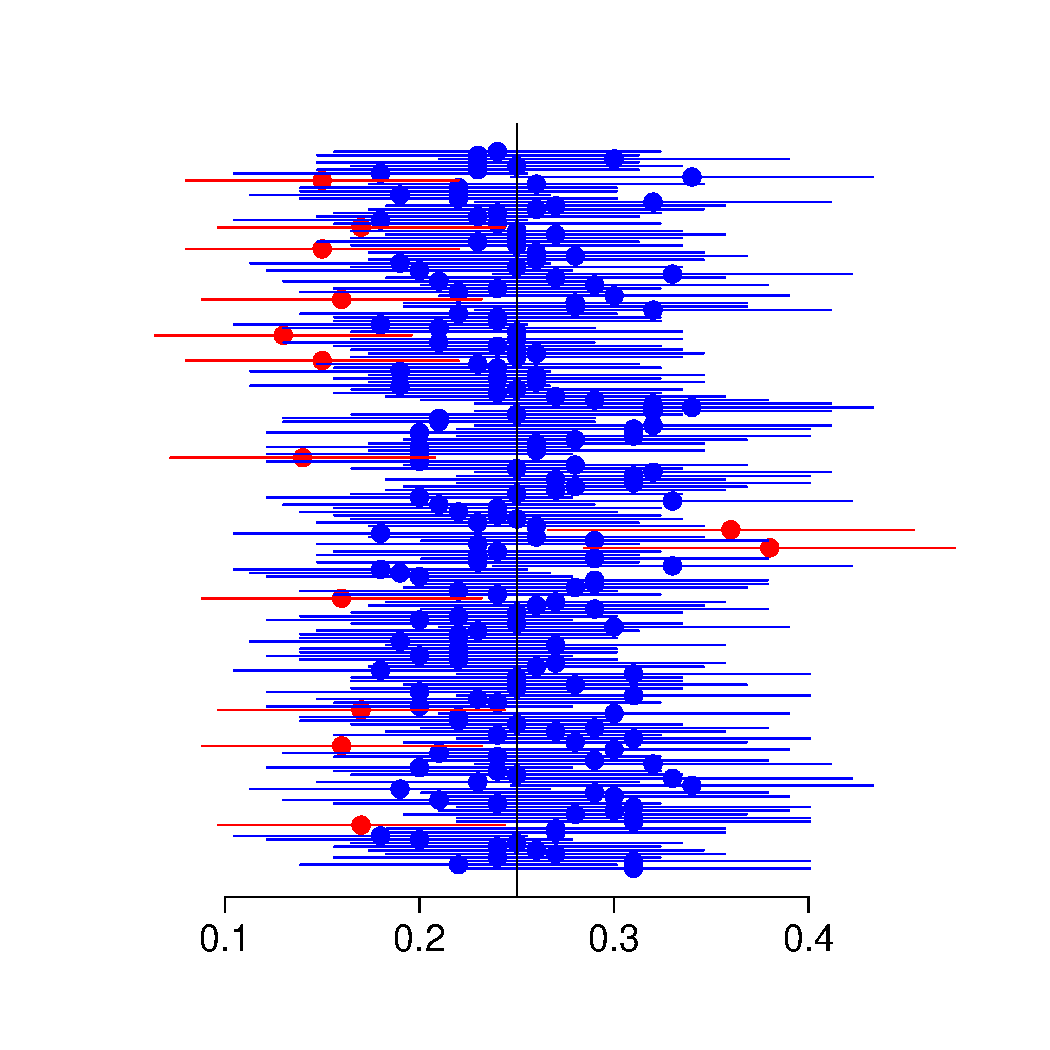
\includegraphics[width=0.65\textwidth]{confi200.pdf}%{overlap3.pdf}
 	\end{figure}
\end{frame}

\begin{frame}{Beobachtete Anteilswerte: 250 Befragungen}
%http://www.faz.net/aktuell/politik/inland/allensbach-umfrage-zeigt-angst-um-innere-sicherheit-steigt-14073805/infografik-sorgen-um-die-14074061.html
  \begin{figure}[ht]
 	\centering
 	      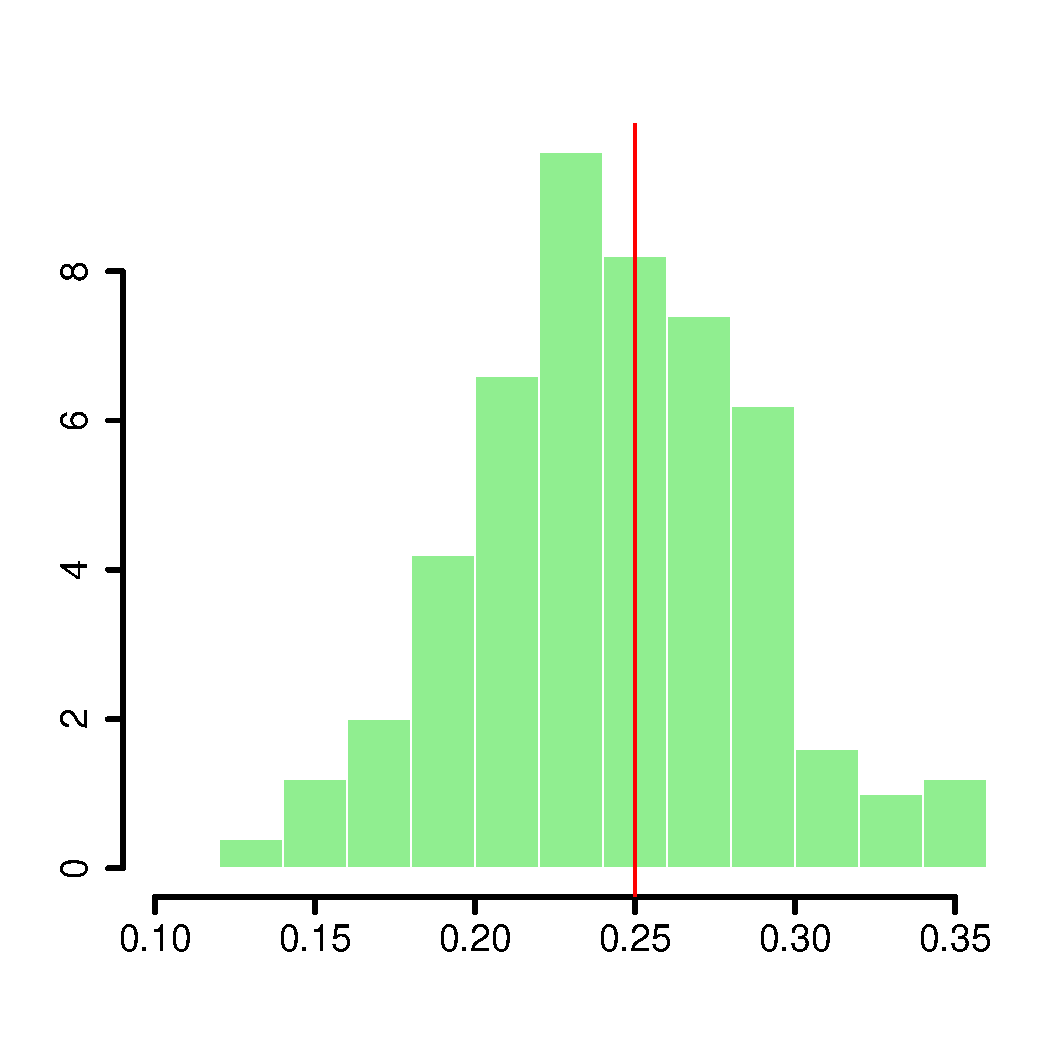
\includegraphics[width=0.65\textwidth]{prob_est250.pdf}%{overlap3.pdf}
 	\end{figure}
\end{frame}

\begin{frame}{Konfidenzintervalle zu den Anteilswerten: 250 Befragungen}
%http://www.faz.net/aktuell/politik/inland/allensbach-umfrage-zeigt-angst-um-innere-sicherheit-steigt-14073805/infografik-sorgen-um-die-14074061.html
  \begin{figure}[ht]
 	\centering
 	      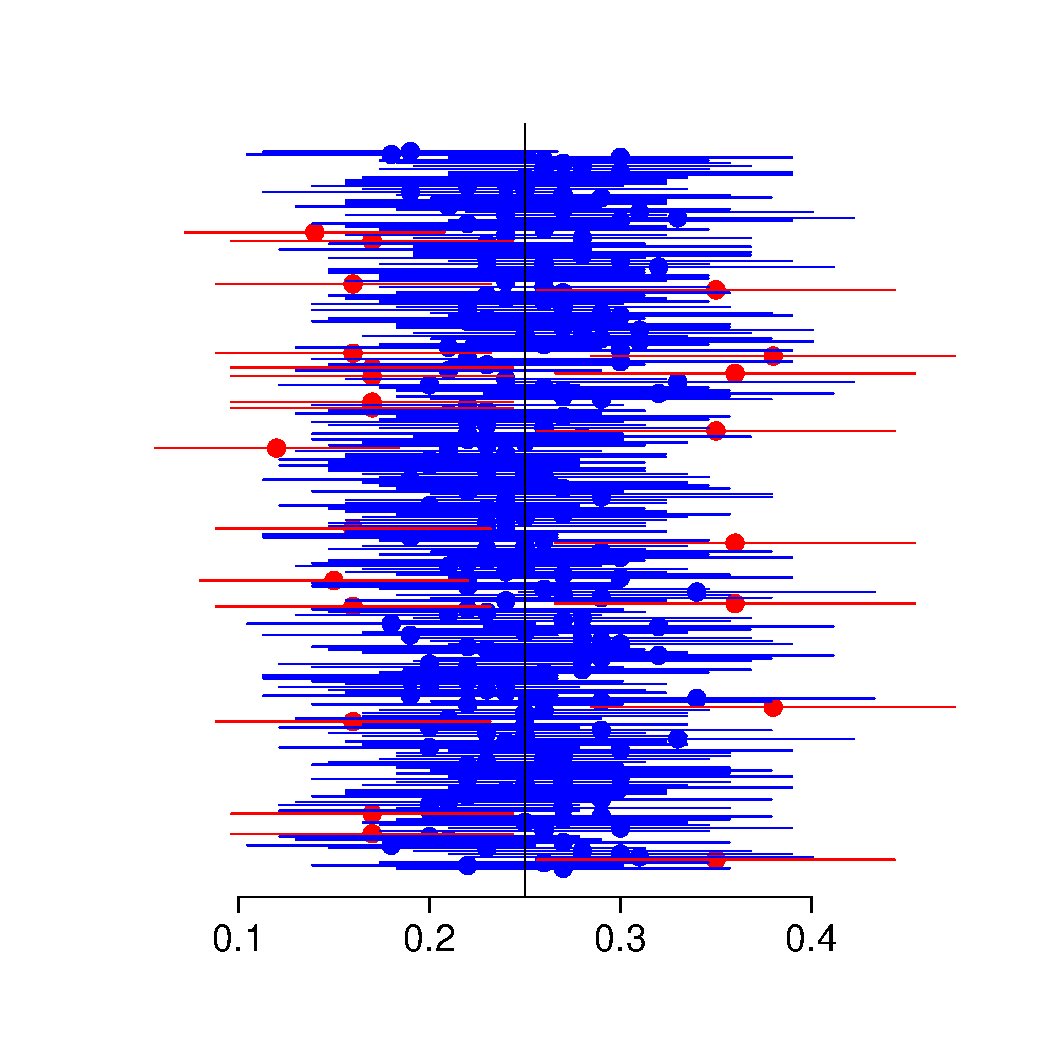
\includegraphics[width=0.65\textwidth]{confi250.pdf}%{overlap3.pdf}
 	\end{figure}
\end{frame}

\begin{frame}{Das zweiseitige $(1-\alpha)$- Konfidenzintervall für $\theta$}
\begin{variableblock}{Das $(1-\alpha)$- Konfidenzintervall für $\theta$}{bg=Orchid!30,fg=black}{bg=Plum!30,fg=black}
Zu vorgegebener Irrtumswahrscheinlichkeit $\alpha$ liefern die aus den Stichprobenvariablen 
$X_{1}, \dots X_{n}$ gebildeten Schätzstatistiken 
$G_{u}=g_{u}(X_{1}, \dots X_{n})$ und $G_{o}=g_{o}(X_{1}, \dots X_{n})$
ein $(1-\alpha)$- Konfidenzintervall (Vertrauensintervall), wenn
gilt
\begin{equation}\label{star} P(G_{u} \leq G_{o})=1 \tag{*} \end{equation}
\begin{equation}\label{star2} P(G_{u} \leq \theta  \leq G_{o})=1-\alpha.  \tag{**}\end{equation}

$1-\alpha$ wird als Sicherheits- oder Konfidenzwahrscheinlichkeit bezeichnet. Das sich aus den Realisationen
$x_{1}, \dots x_{n}$ ergebende realisierte Konfidenzintervall besitzt die Form
$[g_{u},g_{0}],$ wobei 
$g_{u}=g_{u}(x_{1}, \dots x_{n})$ und $g_{o}=g_{o}(x_{1}, \dots x_{n}).$
\end{variableblock}
\end{frame}

\begin{frame}{Interpretation des  $(1-\alpha)$- Konfidenzintervall}
\begin{itemize}
\item{Die obige Definition besagt, dass die Intervallschätzung gerade so
festgelegt ist, dass zwei Dinge erfüllt sind:
\begin{itemize}
\item[1)]{Die untere Intervallgrenze mit Sicherheit niedriger ist als die obere Intervallgrenze (*). Dieser Teil der Definition
ist aus mathematischen Gründen erforderlich und braucht Sie nicht zu interessieren.}
\item[2)]{Vor der Berechnung des Konfidenzintervalls ist die Wahrscheinlichkeit dass man ein Konfidenzintervall
erhält, dass den wahren Parameter nicht enthält eben gleich $\alpha.$(**) Dieser Teil der Definition
ist für die Interpretation grundlegend wichtig.}
\end{itemize}
}\pause
\item{Vor Berechnung des Konfidenzintervalls ist als die Wahrscheinlichkeit ein ``blaues'' Intervall zu bekommen
$(1-\alpha)$ und die Wahrscheinlichkeit für ein ``rotes'' Intervall $\alpha.$}
\end{itemize}
\end{frame}

\begin{frame}{Interpretation des Konfidenzintervalls}
Was bedeutet diese Interpretation für die Praxis:
\begin{itemize}
\item{Wenn Sie ein Konfidenzintervall berechnet haben, dann ist es ein ``blaues'' (enthält $\theta$)
oder ein ``rotes'' (enthält $\theta$ nicht).}\pause
\item{Sie wissen nicht, ob ihr Intervall den wahren Parameter enthält oder nicht.}\pause
\item{Sie wissen, dass es eine Eigenschaft des Verfahrens ist ein Konfidenzintervall zu liefern,
dass in $(1-\alpha)\%$ der Fälle den wahren Parameter enthält.}\pause
\item{Ist das Intervall breit, ist die Schätzung ungenau, ist das Intervall schmal, ist die Schätzung
relativ genau.}\pause
\item{Im allgemeinen gilt, desto größer der Stichprobenumfang desto schmaler das Konfidenzintervall und
desto niedriger die Irrtumswahrscheinlichkeit desto breiter das Intervall.}
\end{itemize}
\end{frame}
\subsection{Äquivalenz von Konfidenzintervallen und Signifikanztests}
%
\begin{frame}{Klassifikation für Tests}
\begin{block}{Parametrische und nicht-parametrische Tests}
Wenn man für die Teststatistik die Kenntnis des Verteilungstyps in der Grundgesamtheit
 voraussetzt, liegt ein parametrischer Test vor, andernfalls ein verteilungsfreier
oder nicht-parametrischer Test.
\end{block}\pause
\begin{itemize}
\item{Der $\chi^{2}$-Test ist ein nicht-parametrischer Test.}
\item{ Alle anderen Tests, die wir bisher behandelt
haben sind parametrisch.}
\item{Wir wollen uns im Folgenden ansehen, warum die Konfidenzintervalle sich als Menge
der beibehaltenen Nullhypothesen interpretieren lassen. Dabei beschränken wir uns
auf ungerichtet Hypothesen, also Hypothesen der Form $\theta=\theta_{0}.$}
\end{itemize}

\end{frame}
%\begin{frame}{Der Punktschätzer}% S. 120 LM, S. 366 FT


\begin{frame}{Der Standardfehler (vgl. LMLG S. 130)}
Um die beiden Interpretationen des Konfidenzintervall aufeinander beziehen zu können,
brauchen wir den Standardfehler für Anteilswerte.
\begin{variableblock}{Definition: Standardfehler }{bg=Orchid!30,fg=black}{bg=Plum!30,fg=black}
Der Standardfehler, of mit der englischen Abkürzung S. E. (für \textit{standard error}) bezeichnet,
ist die Standartabweichung der Schätz- bzw. Teststatistik. Er kann aus den Stichprobendaten
geschätzt werden. In manchen Situationen ist er bekannt und muss nicht geschätzt werden.
\end{variableblock}
\pause
\vspace{0.5cm}
Der Standardfehler hängt u. a. von der Stichprobengröße ab: Große Stichproben produzieren
unter sonst gleichen Bedingungen geringe, kleine Stichproben produzieren hingegen große
Standardfehler.
%\begin{itemize}
%\item{Um die beiden Interpretationen des Konfidenzintervall aufeinander beziehen zu können,
%brauchen wir den Standardfehler für Anteilswerte}%LMLG S. 133
% Äquivalenz S. 165
%\end{itemize}
\end{frame}



\begin{frame}{Konstruktion eines Konfidenzintervalls}
Wenn die Verteilung des Schätzers zur Familie 
der Normalverteilungen gehört, sind Konfidenzintervalle nach dem folgenden Muster gebaut: 
$$\hat{\theta} \sim N\big(\theta, \hat{\sigma}_{\hat{\theta}}\big)$$%N(\theta,\hat{\sigma}_{\hat_{\theta}})
oder 
$$\hat{\theta} \sim N\big(\theta, \sigma_{\hat{\theta}}\big)$$ wenn der S. E. $\sigma_{\hat{\theta}}$
bekannt ist.
\begin{itemize}
\item[1)]{Die untere Grenze $G_{u}$ wird berechnet als $\hat{\theta}-z_{1-\frac{\alpha}{2}}\cdot S.E.$}
\item[2)]{Die untere Grenze $G_{o}$ wird berechnet als $\hat{\theta}+z_{1-\frac{\alpha}{2}}|\cdot S.E.$}
\end{itemize}
dabei ist $z_{1-\frac{\alpha}{2}}$ das $1-\frac{\alpha}{2}$ Quantil der Standardnormalverteilung und
S. E. ist der bekannte oder geschätzte Standardfehler des Schätzers $\hat{\theta}.$
\end{frame}
%
%\begin{itemize}
%\item{mit $\hat{\theta}:$ Schätzwert für den Parameter}
%\item{$q_{\frac{alpha}{2}}$ bzw. $q_{1-\frac{alpha}{2}}:$ Quantile der Standardnormalverteilung}
%\item{S. E.: Standardfehler des Schätzers}
%\end{itemize}

\begin{frame}{Standardfehler für Anteilswerte I}
\begin{itemize}
\item{Der Schätzer $\hat{p}$ ist asymptotisch normalverteilt.}
\item{Asymptotisch bedeutet,
dass man bei großen Stichprobenumfängen von einer Normalverteilung ausgehen darf.}
\item{Daher steht in der FS S. 52 die Voraussetzung $n \cdot p (1-p) \geq 9.$}
\item{Unter dieser Voraussetzung gilt: $$\hat{p} \sim N (p, \hat{\sigma}_{\hat{p}}),$$
mit $$\hat{\sigma}_{\hat{p}}=\sqrt{\frac{\hat{p}(1-\hat{p})}{n}}.$$}%=\sqrt{\frac{\hat{p}(1-\hat{p})}{n}}$$
%}
\end{itemize}
 
\end{frame}

\begin{frame}{Standardfehler für Anteilswerte II}
Der Schätzer $\hat{p}$ ist asymptotisch normalverteilt
$$
\hat{p} \overset{a}{\sim} N\big(p, \hat{\sigma}_{\hat{p}}\big).
$$
Gemäß dem obigen Konstruktionsprinzip ergibt sich dann genau
das Konfidenzintervall \eqref{eq:1}, also
$$
\bigg[\hat{p} - z_{1-\frac{\alpha}{2}}\Bigg(\sqrt{\frac{\hat{p}(1-\hat{p})}{n}}\Bigg),\hat{p} + z_{1-\frac{\alpha}{2}}\Bigg(\sqrt{\frac{\hat{p}(1-\hat{p}}{n}}\Bigg) \Bigg].
$$
\end{frame}

\begin{frame}{Äquivalenz von Konfidenzintervallen und Signifikanztests}
Die Teststatistik im approximativen Binominaltest ist (vgl. FS S. 57) $$T = \frac{\hat{p}-p_{0}}{\sqrt{p_{0}(1-p_{0})}}\cdot \sqrt{n}. $$%
\begin{itemize}
\item{h}
\end{itemize}
\end{frame}

%\begin{frame}{Das Konfidenzintervall: Die häufigste Interpretation}% S. 125
%\end{frame}
% Stichprobenverteilung mit Verweise auf LMLG
% Def: Konfidenzintervall
% Zurück zum Beispiel
%\begin{frame}{Allensbach-Umfrage : 100 Befragungen}
%http://www.faz.net/aktuell/politik/inland/allensbach-umfrage-zeigt-angst-um-innere-sicherheit-steigt-14073805/infografik-sorgen-um-die-14074061.html
%  \begin{figure}[ht]
% 	\centering
% 	      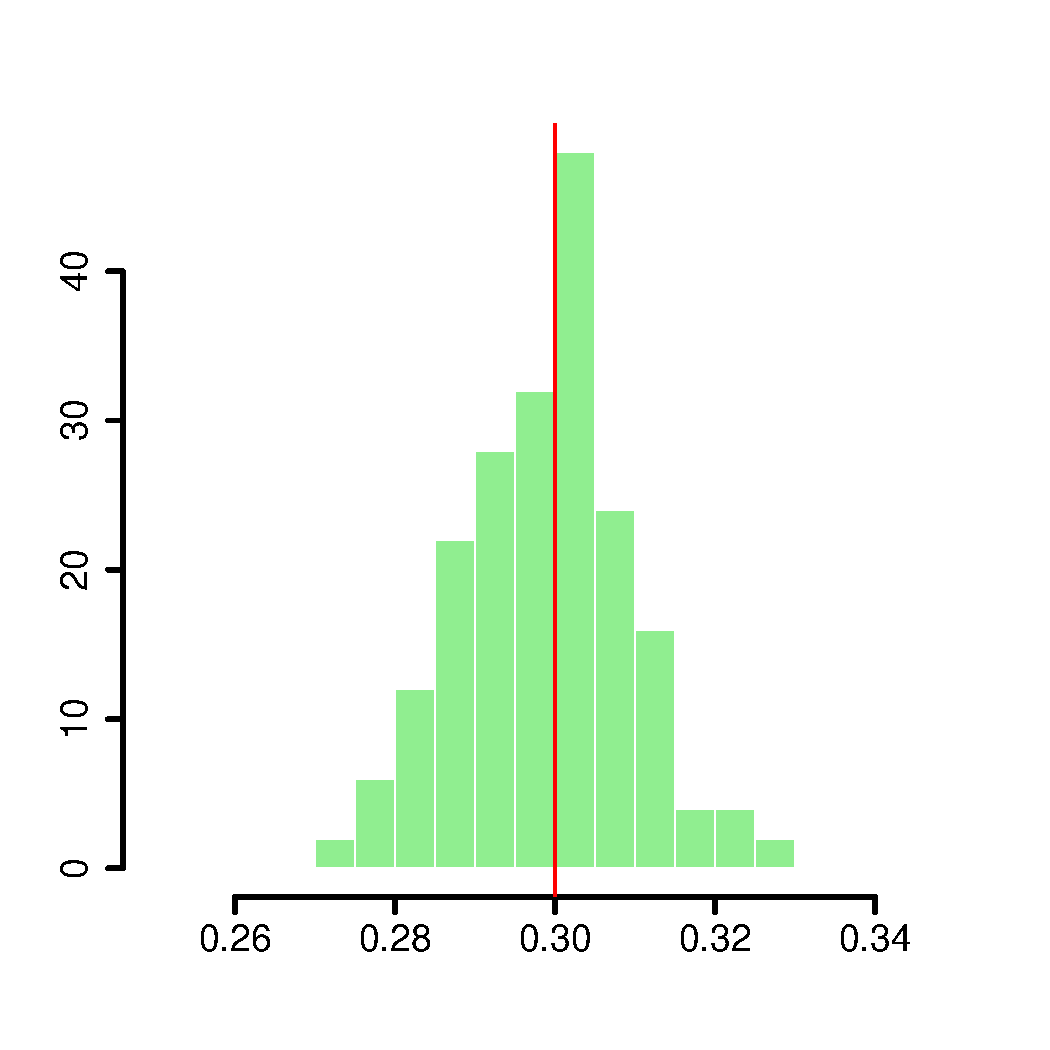
\includegraphics[width=0.65\textwidth]{umfrageEst.pdf}%{overlap3.pdf}
% 	\end{figure}
%\end{frame}
\section{Ausblick: Übung}
%\begin{frame}{Allensbach-Umfrage: 100 Befragungen}
%%http://www.faz.net/aktuell/politik/inland/allensbach-umfrage-zeigt-angst-um-innere-sicherheit-steigt-14073805/infografik-sorgen-um-die-14074061.html
%  \begin{figure}[ht]
% 	\centering
% 	      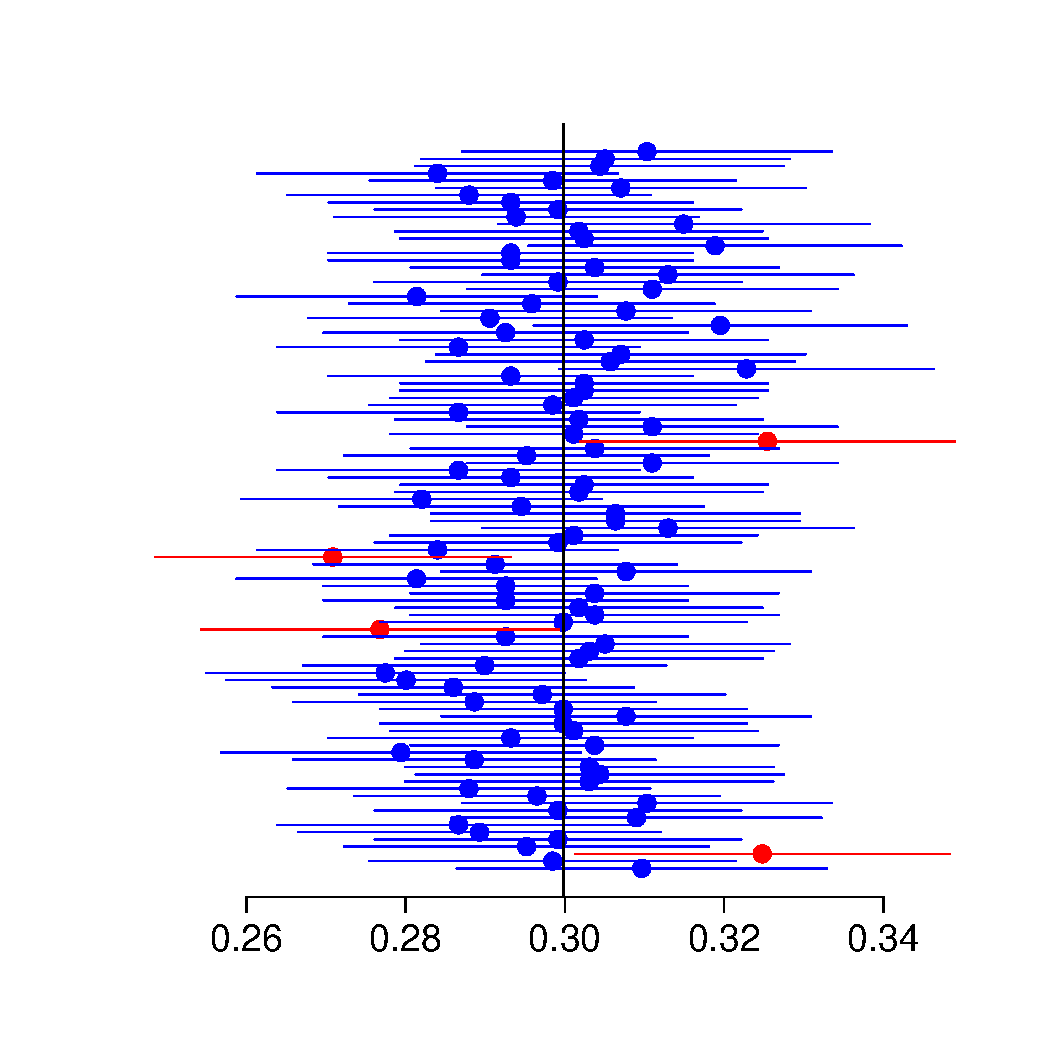
\includegraphics[width=0.65\textwidth]{umfrageConfi.pdf}%{overlap3.pdf}
% 	\end{figure}
%\end{frame}
% Man beachte: Es sind genau so viele falsch, aber das Intervall ist kürzer.
% Zu den paprametrischen Test gibt es auch ein entsprechendes Konfidenzintervall
% chi-2 ist nicht parametisch...


%http://www.statistik-und-beratung.de/2013/07/statistischer-vergleich-von-zwei-gruppen/
\begin{frame}{Ausblick: Übung}
 \begin{figure}[ht]
 	\centering
 	      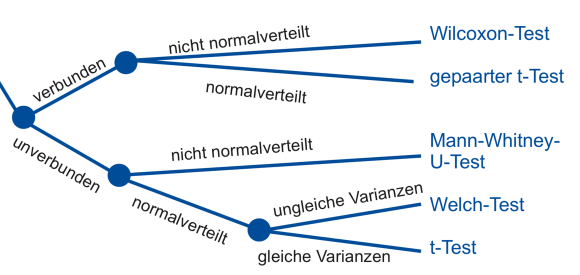
\includegraphics[width=0.95\textwidth]{Test_EB.png}%{overlap3.pdf}
 	      \caption{Quelle: \url{http://www.statistik-und-beratung.de/2013/07/statistischer-vergleich-von-zwei-gruppen/}}
 	\end{figure}
\end{frame}


% Wilcoxon Test S. 157
\begin{frame}{Ausblick: Übung}
\begin{itemize}
\item[1)]{Wir schauen uns die Teststärke und das Konfidenzintervall an, um die 
Frage ob Mädchen besser lesen als Jungs, klären zu können.}\pause
\item[2)]{Der Begriff nicht-parametrischer Test wird erklärt. Der $\chi^{2}$-Test
ist ein nicht-parametrischer Test. Zwei weitere wichtige Tests sind der U-Test und der
Wilcoxon-Test. Diese werden vorgestellt. Bei den nicht-parametrischen Tests ist es nicht möglich den Test durch die Berechnung
eines Konfidenzintervalls zu umgehen.}\pause
\item[3)]{Wir lernen den Q-Q-Plot kennen, als Methode um zu Entscheiden, ob es sinnvoll
ist von einer Normalverteilung auszugehen, oder nicht.}\pause
\end{itemize}
\end{frame}
\end{document}

